% +++
% sequence = ["latex", "bibtex", "latex", "latex"]
% [programs.latex]
% 	command = "lualatex"
% 	opts = ["-synctex=1", "-file-line-error", "-interaction=nonstopmode"]
% 	args = ["%S"]
% [programs.bibtex]
% 	command = "upbibtex"
% 	target = "../ref.bib"
% 	args = ["%B"]
% +++

\documentclass[./main]{subfiles}
% \graphicspath{{\subfix{./figures/section2/}}}
\setcounter{section}{1}

\begin{document}
\section{\TeX と \LaTeX}
\addtocontents{lof}{\protect\addvspace{1em}}

\noindent
まず,\TeX と \LaTeX は異なるものである.
しかし,そもそも名前が似てるし,両者の区別が曖昧のままでも所望の文書を作成することはとりあえずできてしまうので,別にどっちでもいいという考え方もできる.
が,違いがあるから名前が違うのである.
ここでは \TeX と \LaTeX の何が違うのかを説明し,言葉として\TeX がつく様々なものについて,今後混乱・誤用しないようにざっくりと解説していく.

ところで,\TeX は\TeX であり,\verb|tex|でも\verb|TEX|でもなければ\verb|Tex|でもない.
しかし,場合によってTeXと表記されることはある.
また,本資料では拡張子が \verb|*.tex|となっているものについては\verb|tex|ファイルなどと表記することにする.
\LaTeX も同様で,\LaTeX かもしくはLaTeXである.
ちなみに,\TeX の発音はアルファベットのX \textipa{/\textepsilon ks/}として読むのではなく,無声軟口蓋摩擦音\textipa{/x/}と発音するのが正しい(諸説あるが)\footnote{
  日本語で表記するなら「てふ」であり,歴史的仮名遣い的にその発音は\textipa{/t\textesh o\textlengthmark/}である.
}.

\subsection{\TeX とはなにか}
\noindent
\TeX とは1978年に Donald E. Knuth\supercite{KnuthHP} が発表した``組版\footnote{原稿及びレイアウトの指定に従って,文字・図版・写真などを配置する作業の総称\supercite{Typesetting_Wikipedia}.}ソフトウェアと組版言語''である\supercite{reutenauer2008brief}\footnote{由来はギリシャ語で美術や工芸を意味する``\texttau\'{\textepsilon}\textchi\textnu\texteta''\textipa{/t\'{e}xni/}}.
つまり,``文章そのもの''と``文章の構造を指定する命令''が書かれたテキストファイル(この命令を記す言語も\TeX という)を読み込み,その命令に従って文章を組版するソフトウェアが\TeX である.
組版結果はDVI形式 (DeVice-Independent) に書き出されるが,この\verb|dvi|ファイルは文書の見た目のレイアウト(紙面のどの位置にどの文字を配置する,などの情報)を画像形式・表示デバイス・プリンタにまったく依存しない形で記録している\supercite{TeXdiff_wtsnjp}.
結局\TeX をとてもざっくりまとめると(Knuthの思う)美しい組版がデバイスによらない形式で出力される,ということになろう.

\subsection{\LaTeX とはなにか}
\noindent
\TeX での命令は「横方向に何センチメートルの空白を作る」のように非常に原始的なものなので,
使い勝手が良くない.
そこで\TeX を使ってもっと簡単に論文やレポートを作成したいという要望から \LaTeX は開発された\supercite{LaTeX_TeXWiki}.
\TeX の原始的な命令を組み合わせて新しい命令(マクロ)を作ることができる(\verb|\def|みたいなやつ)が,\TeX で文書作成する際には多量のマクロが必要になるため,それらの必要なマクロが一通り揃えられた``マクロ体系''の1つが \LaTeX である.

繰り返しになるが,この世にいくつも存在する\TeX を楽に使うためのマクロ体系のひとつが\LaTeX である.
現代の多くの\verb|tex|ファイルはマクロが準備された\LaTeX で処理されることが前提であり,それを\TeX で処理しようとして目的のものが得られることはまずない.
次節で述べる通り,\TeX にも\LaTeX にも沢山の種類がある.
つまり,同じ\LaTeX でも\pLaTeX と\LuaLaTeX とでは用意されているマクロや定義に違いがあるため,\verb|tex|ファイルが想定するそれと処理する\LaTeX が食い違っていればエラーが出るのも当然である.
また,\LaTeX で定義されたマクロのおかげで成り立つ事象を\TeX 全体で成り立つと理解するのは危険なのである.

\subsection{その他のナントカ\TeX とか\TeX ナントカとかナントカ\TeX ナントカとはなにか}
\noindent
\TeX と\LaTeX 以外にも名前に\TeX がつくものは数多くある.
違いがわかるように簡単にまとめておこう\supercite{TeXwiki}.

\subsubsection{\TeX の仲間}
\noindent
組版を行うソフトウェアとして,もともとの\TeX の機能が様々に拡張されたものがある.
例えば,
\begin{itemize}
  \item \eTeX : オリジナルの\TeX と100\% の互換性を保ちながら\TeX の少々不便なところを補う実用性の高い拡張.
  \item \pTeX : 縦組みに対応し,和文組版できる拡張\TeX.
  \item \epTeX : \eTeX を取り入れた\pTeX.
  \item \upTeX : \pTeX のUnicode\footnote{様々な言語の文字を単一の文字コードで取り扱うために開発されている文字コード\supercite{Unicode_Wikipedia,師茂樹2009unicode}}版.
  つまり,\pTeX の内部コードをUnicode化している.
  簡単に言ってしまえば扱える文字が増える.
  例えば\figref{fig:pTeX_vs_upTeX}では同じ日本語で書かれた\verb|tex|ファイルを\pTeX と\upTeX で処理した際の出力の違いである(正確には\pTeX に対応したマクロ体系\pLaTeX を利用した場合と\upLaTeX を利用した場合の違い).
  \pTeX の方では一部の文字(例えば踊り字「〻」や非常用漢字「沆瀣」など)が出力されていないことがわかる.
  Unicodeを用いることでこの世に存在するより幅広い文字を扱えることになる.
  \item \pdfTeX : \eTeX の拡張.DVIではなく,PDFを直接出力する.
  少しだけ触れたが,\verb|dvi|ファイルとはデバイスに依存しない,\TeX 固有の出力形式である.
  人間が読めるようになっているわけではないため,別にPDFなどに変換する操作(\verb|dvipdfmx|とかそういうの)が必要である.
  \pdfTeX は出力としてこの\verb|dvi|ではなく\verb|pdf|ファイルを直接出力するため,そういった変換も不要なほか,ハイパーテキストリンクや目次といったPDFの機能を直接扱うことができる.
  \item \XeTeX (\textipa{/zi\textlengthmark t\textepsilon x/})\supercite{XeTeX_Wikipedia,XeTeX_TeXWiki} : \eTeX の拡張.
  符号空間をUnicode全体に拡大したもの(上述\upTeX の説明参照).
  また,OpenTypeフォントに対応している.
  これはつまり,OSにインストールされているフォントをそのまま利用することが可能ということである\supercite{XeTeX_nopoleos}.
  もともとの\TeX では組版を行うとき,組み立てる文字の情報を\verb|tfm|ファイルと呼ばれるものから参照する.
  したがって好きなフォントを使うためにはそのための\verb|tfm|ファイルを用意する必要があったのだが,\XeTeX ではその必要はなく,インストールさえしてしまえば好きなフォントが使える.
  \item \LuaTeX : \pdfTeX の後継.
  OpenTypeフォント,Unicodeに対応しているほか,Luaという軽量スクリプト言語を利用できる.
  このLuaの利用によりあらゆるものがカスタマイズ可能となり,究極の柔軟性が得られる\supercite{八登2010日本人}.
  % (to-do) Luaを使ったおもちゃをいくつかとフォントの切り替えの楽さの確認.
\end{itemize}
\begin{figure}[btph]
  \centering
  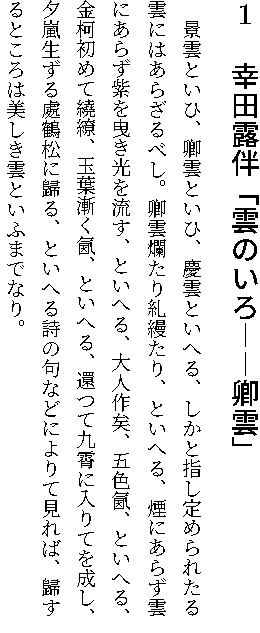
\includegraphics[width=0.25\linewidth]{kumo_p_cmpr.pdf}
  \hspace{0.1\linewidth}
  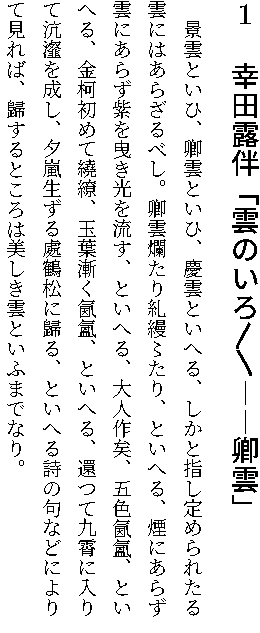
\includegraphics[width=0.25\linewidth]{kumo_up_cmpr.pdf}
  \caption{\pTeX\ engine (left) vs \upTeX\ engine (right).\supercite{幸田1987雲}}
  \label{fig:pTeX_vs_upTeX}
\end{figure}

\clearpage
\subsubsection{\LaTeX の仲間}
\noindent
\TeX を使いやすくするためのマクロ体系は\LaTeX 以外にもあって,例えば以下のようなものがある:
\begin{itemize}
  \item plain \TeX : Knuth 自身が開発したもので,組版に最低限必要となる程度の機能しか持たない.
  \item \pLaTeX : \pTeX に対応した\LaTeX.
  \item \upLaTeX
  \item \pdfLaTeX
  \item \XeLaTeX
  \item \LuaLaTeX
  \item \ConTeXt : 文書の体裁もユーザー自身によってすべて調整可能とすることを目標としているマクロ体系\supercite{ConTeXt_TeXWiki}.
  外部パッケージなしであらゆる部分の調整が可能となるようになっているため,\LaTeX で起こるようなパッケージ同士の衝突などはおこらない.
  \figref{fig:ConTeXt_test}に\ConTeXt を使った\verb|tex|ファイルの例とその出力\verb|pdf|ファイルを示す.
  左のコードの中で赤く示した命令(\verb|\starttext|と\verb|stoptext|)の間が本文であり,その前がいわゆるプリアンブルである.
  パッケージ等を用いず,すべての設定をユーザー自身が行う必要があり,プリアンブルが長くなっている印象である.
  一方,体裁は自分で好きなように決められることがそもそものコンセプトなので,セクション(\ConTeXt 的には\verb|\subject|)の色や図の位置などの調整は自由かつ思い通りに扱いやすい.
\end{itemize}
\begin{figure}[hbbp]
  \centering
  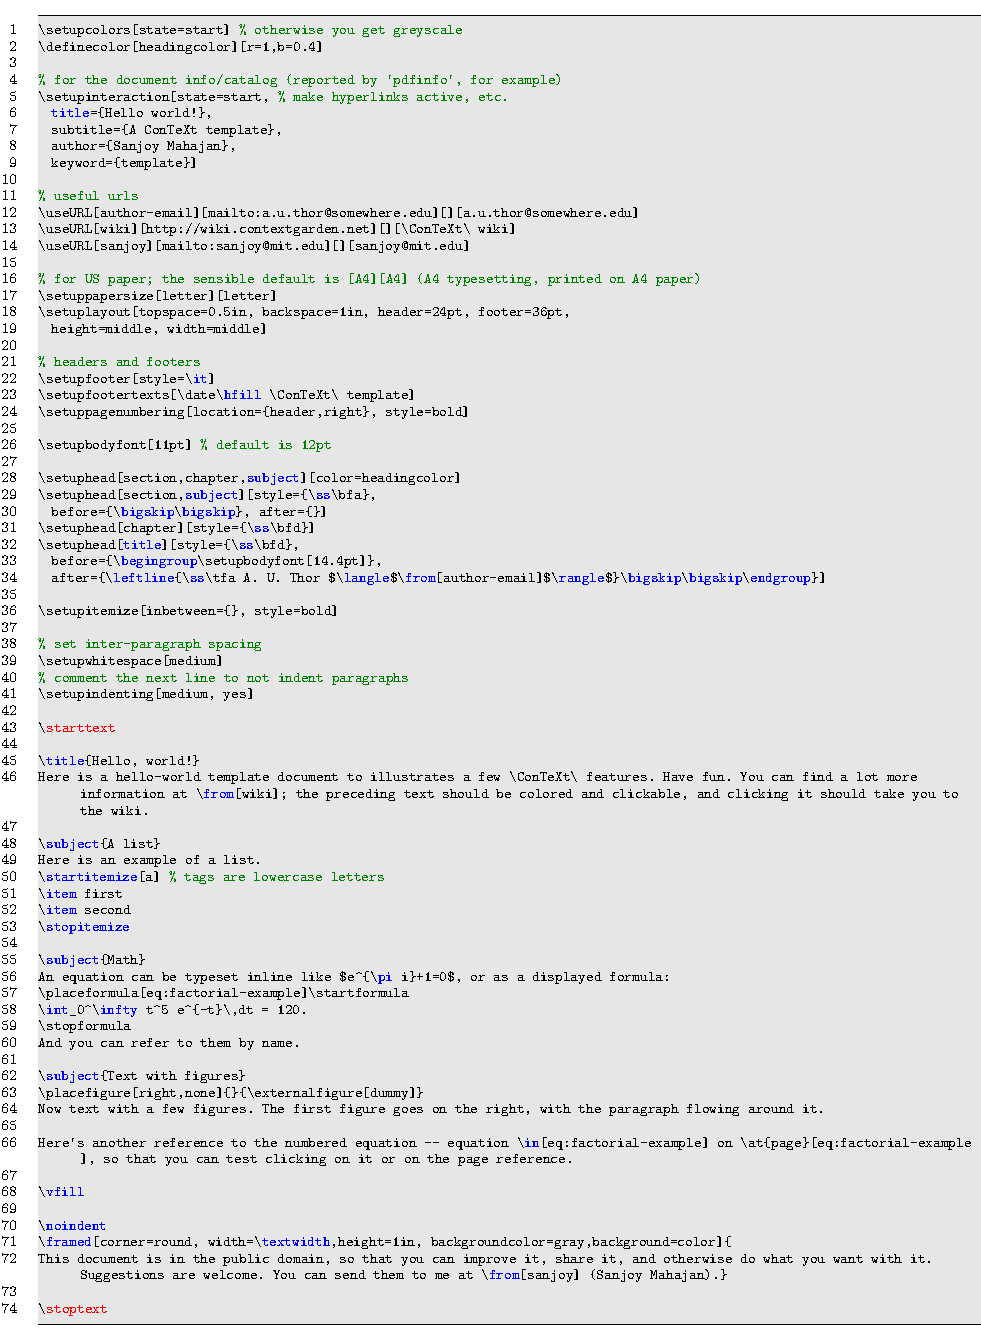
\includegraphics[width=0.4\hsize]{ConTeXt_code.pdf}
  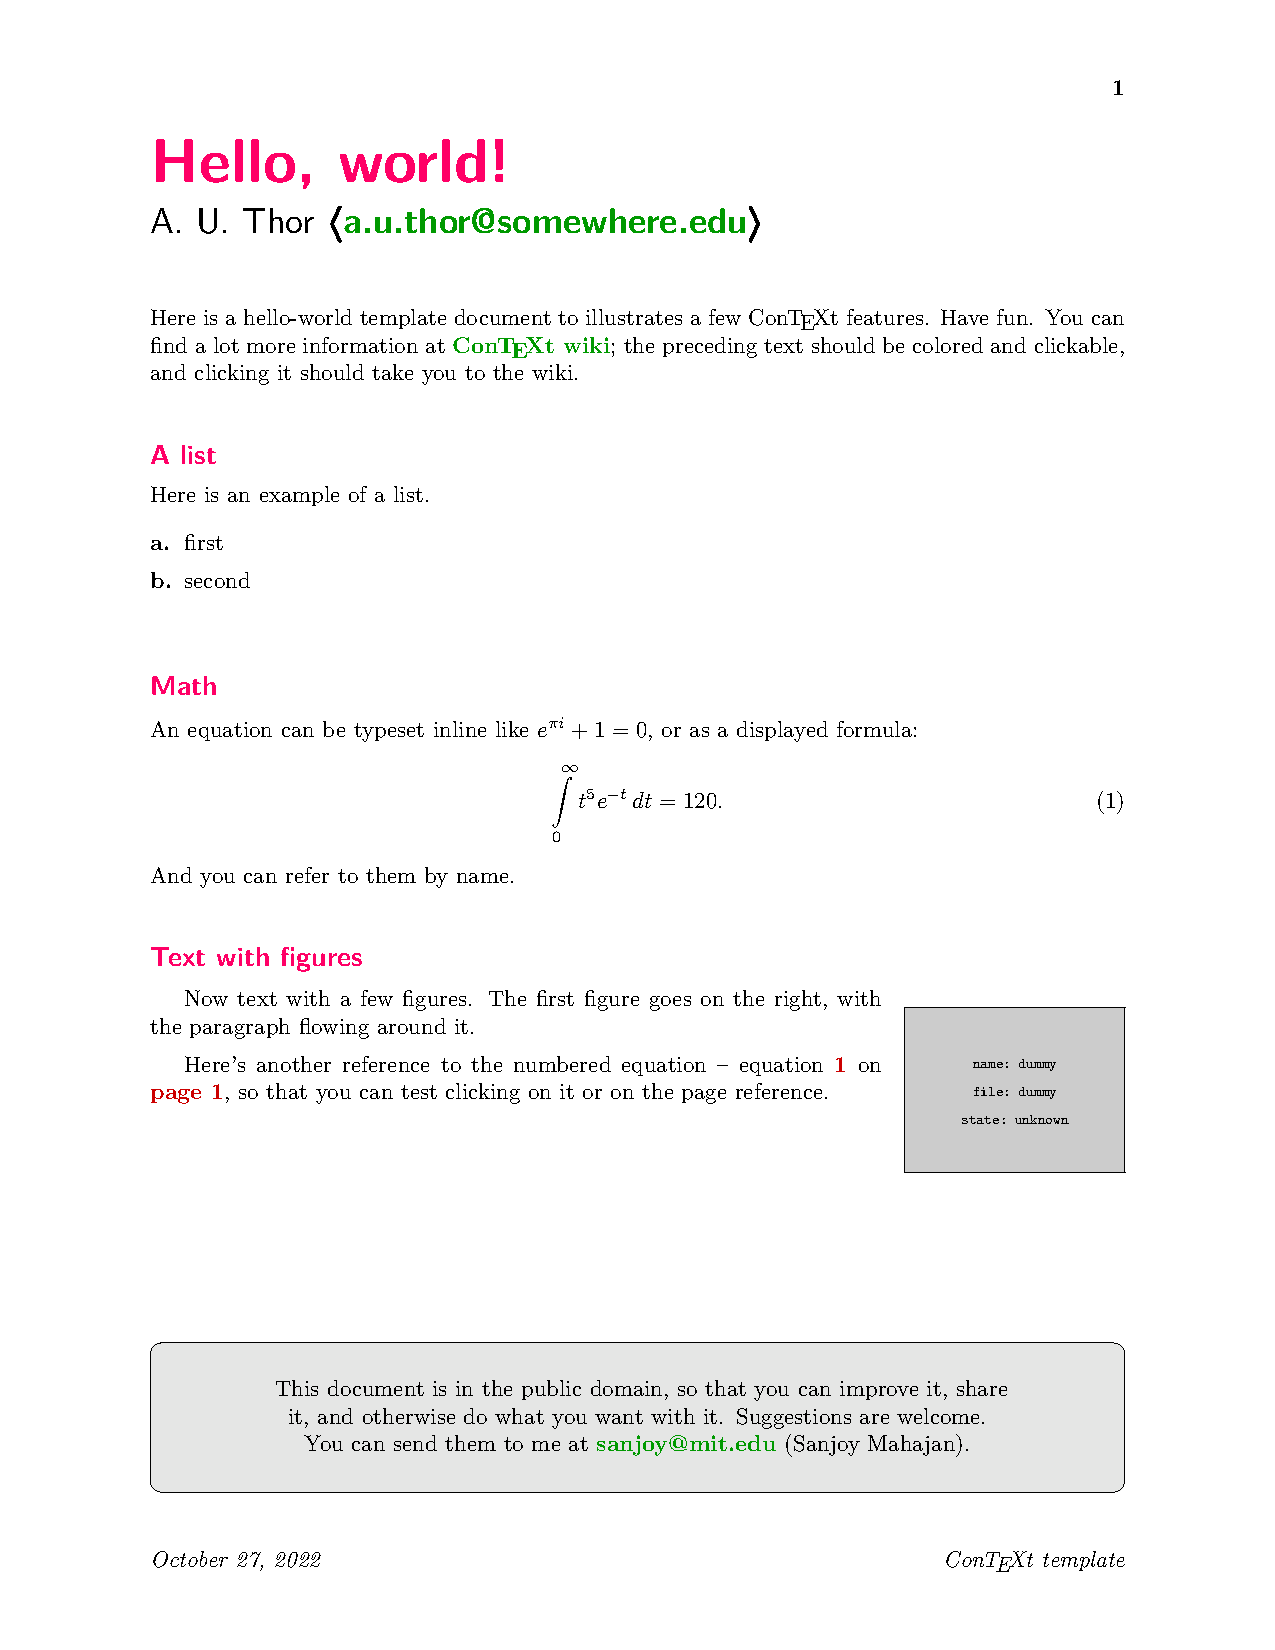
\includegraphics[width=0.4\hsize]{ConTeXt_test.pdf}
  \caption{Example of \ConTeXt\ (left: source tex file, right: pdf file)}
  \label{fig:ConTeXt_test}
\end{figure}

少し話は変わるが,\LaTeX のバージョンについても名前がついている:
\begin{itemize}
  \item \LaTeXe : 現在({\DTMsetdatestyle{default}\today})の主流.
  \item \LaTeX 2.09: 古いバージョン.
  \item \LaTeX 3: 開発中の次期バージョン.
\end{itemize}

ここまで,組版ソフトウェアの\TeX とその拡張,\TeX を楽に使うためのマクロ体系の\LaTeX とその拡張および仲間について説明した.
ここからは\TeX の名前がついていて,\TeX とともに使うもの\footnote{\LaTeX は\TeX\,``を''使うもの}について見ていこう.

\subsubsection{文献管理ソフト}
\noindent
\verb|\cite|等を使って文献の引用をする場合,そのタイトルや著者,出版年,出版社等々の文献情報を管理しなくてはならない.
\verb|thebibliography|環境でひとつずつ(\verb|\bibitem|)自分の手で文献情報を入力することも可能だが,数が増えると大変である上,表記に一貫性を持つための調整も手間である.
そんなときに,\LaTeX と組み合わせて文献データベースから自動的に参考文献リストを作るためのツールが文献管理ソフトである.
よく耳にするのは
\begin{itemize}
  \item \BibTeX : 書誌情報のデータベース(\verb|bib|ファイル)を用いて,自動で参考文献リストを作成する.
  このデータベース\verb|bib|ファイルのなかで各書誌情報はまずエントリごとに種別分けされ(\verb|@article|, \verb|book|, \verb|proceedings|, etc.) ,それぞれの情報を保存する(\verb|title|, \verb|author|, \verb|journal|, etc.).
  \item \pBibTeX : \pTeX に特化.日本語の文献を扱える.
  \item \upBibTeX
\end{itemize}
などがあるが,最近は他にも
\begin{itemize}
  \item Bib\LaTeX (+\verb|Biber|) : \LaTeX で用いるパッケージ.
  そもそも\BibTeX は参考文献のフォーマットは\verb|bst|ファイルというもので設定されるのだが,これまた編集が大変である.
  そのため,よりカスタマイズが容易なのが,本パッケージである.
  Bib\LaTeX のバックエンド(文献のソートを担当)として\verb|biber|か\verb|bibtex|を用いることになるが,\verb|biber|のほうが\verb|bibtex|を用いるよりさらにカスタマイズの柔軟性が上がる\supercite{Biber_Wikipedia}.
\end{itemize}
が次世代文献管理ソフトとして挙げられる.

\subsubsection{統合開発環境}
\noindent
\TeX 周りの作業がしやすいように整備されたエディタ.これさえあれば\TeX がつかえる,というものではない.
\begin{itemize}
  \item \TeX Shop: macOS専用の\LaTeX 統合環境.シンプルなUIと直感的な操作性が特徴.
  \item \TeX works: \TeX Shopをモデルにすべてのシステム上で実現すべく開発された\LaTeX 用統合環境.
  \item \TeX studio: 豊富な機能と高度なLaTeXサポートがあり,拡張性が高い.全システム上で動く.
\end{itemize}

\subsubsection{ディストリビューション}
\noindent
\TeX がまともに使えるようになるためには\TeX さえあればいい,わけではない.
\TeX なのか\pTeX なのか\LuaTeX なのか.\LaTeX なのか\ConTeXt なのか.
\BibTeX なのか\verb|Biber|なのか.
統合開発環境は使うのか.使うならどれか.
さらに言えば,自分の文書作成では\LuaLaTeX のみ使うと決心したとしても,学会によっては\upLaTeX で動くことのみ想定したフォーマットを配っている場合もあり,そのフォーマットを\LuaLaTeX 用に書き換えるのはただ面倒で生産性があまりなく,こうなると最初から\upLaTeX を準備しておくのが望ましい.
これ以外にも,特定のマクロ体系を更に拡張するための``パッケージ''が必要なことがほとんどで,それらも新たに必要になるたびインストールしなくてはならない.
結局,\TeX を使えるようになるためには非常に多くのものをインストールしなくてはならないが,一つ一つ個別にインストールするのは大変であり,これらを一括でインストールできるのがディストリビューションである.

日本国内で多く用いられているディストリビューションは
\begin{itemize}
  \item \TeX Live\supercite{TeXLive_Acetaminophen}
\end{itemize}
であるが,他にも
\begin{itemize}
  \item Mac\TeX : \TeX LiveをベースにしたmacOS専用のディストリビューション.
  \item Basic\TeX : \LaTeX の文書作成に必要最低限なものが含まれるmacOS専用ディストリビューション.\epTeX などが含まれない.
  \item MiK\TeX : Windows,macOS,Linuxで動作するディストリビューション.日本語\pTeX が含まれない.
\end{itemize}
などが存在する.


\subsection{番外編:文書クラス}
\noindent
さて,\TeX と名のつくものについて説明してきたが,ここで\TeX を名前に含まないものの,種類がいくつかあってややこしいものとして,文書クラスについて解説する\supercite{documentclass_list}.
\verb|tex|ファイルの一番最初に\verb|\documentclass|とか書くあれである.
\begin{itemize}
  \item \verb|article|: 論文やレポートなどの一般的な文書.
  文章の構造は\verb|part|, \verb|section|, \verb|subsection|, \verb|subsubsection|, \verb|paragraph|, \verb|subparagraph|の6つのレベルに分けられる.
  \item \verb|report|: 論文やレポートのより長い文書.
  構造としては\verb|article|に\verb|chapter|が追加される(\verb|part|と\verb|section|の間).
  また,(デフォルトの設定では)\verb|part|が$1$ページ使って表示される(Part I 〇〇とだけ書かれたページができる).
  \item \verb|book|: 書籍.構造は\verb|report|と同じだが,奇数ページと偶数ページのレイアウトが変わる.
  例えば,\verb|part|の示すページは必ず奇数ページ(見開きの右側)になる.
  \item \verb|jarticle|: 和文横書き対応の\verb|article|.
  \item \verb|jreport|
  \item \verb|jbook|
  \item \verb|tarticle|: 和文縦書き対応の\verb|article|.
  \item jsclasses (\verb|jsarticle| etc.): 日本語(u)\pLaTeX 用の新しい文書クラス\supercite{jscls_doc}.JISフォントメトリックを使用している.簡単に言えば「文字の組み方」が綺麗に,読みやすくなる.例えば「ちょっとチャックをチェック」のように小さい文字を並べて表示する際\verb|jarticle|などのmin10フォントメトリックでは不自然に詰められ,美しくなかったり読みづらかったりするのがjsclassesでは解消される\supercite{LaTeX_are}.他にも日本語中の英語の組み方などに差が出る.
  \item ltjsclasses (\verb|ltjsarticle| etc.): jsclassesを\LuaLaTeX 用に改変したもの.
  \item bxjsclasses (\verb|bxjsarticle| etc.): jsclassesの派生で,(u)\pLaTeX 依存の部分を切り離したもの.つまり,\LuaLaTeX など他のエンジンを用いても綺麗な日本語文書を作成できる.
  \item \verb|jlreq|: 「日本語組版処理の要件」\footnote{
    標準化団体W3C (World Wide Web Consortium) の技術ノート``Requirements for Japanese Text Layout''\supercite{Req4JapTex,JIS_X_4051}のことで,字詰めやルビ,ページ構成や図表に関してなどあらゆる規定が書かれている.
  }を満たす\LuaLaTeX,(u)\pLaTeX 用の文書クラス.
  \item \verb|beamer|: スライド.「Beamerのすゝめ」も読んでね.
\end{itemize}


\ifSubfilesClassLoaded{%
  \printbibliography
}{}

\end{document}
